\documentclass[12pt,a4paper]{article}

\usepackage{ctex}

\title{写字板设计报告}
\author{计24班{} 田博{} 2012011346{} 楼华哲{} 2012011327}

\begin{document}
\maketitle

\section{实验目的}
通过VHDL语言在FPGA上实现一个类似Windows写字板的写字板程序。主要有以下功能:

\begin{itemize}
	\item 字符任意位置插入、删除,字符集包括所有ASCII码可见字符;
	\item 字符和按钮清晰显示,完全不存在毛刺;
	\item 文本选中,通过按钮设置大小、字体、颜色;
	\item RAM存储文本,强扩展性,理论支持任意长度文本;
	\item 支持文本翻页功能;
	\item 表情符号(emoji)插入模式。
\end{itemize}

\section{整体设计} % (fold)
\label{sec:整体设计}
为了实现丰富的功能,我们主要有以下模块:

\begin{itemize}
	\item GlobalDefines.vhd,定义全局的常量信息。
	\item TextProcessor.vhd,响应键盘和鼠标事件,根据用户操作和当前文本状态对RAM中的文本进行修改。
	\item TextDisplayer.vhd,结合文本状态和当前RAM中的内容绘制屏幕。
	\item PS2KBInterface.vhd,将PS2信号转化为scancode。
	\item KeyScanner.vhd,将scancode转化为ASCII码。
	\item VGADisplayer.vhd,控制VGA显示,提供当前扫描坐标,接受TextDisplayer的颜色来显示。
	\item ps2\_mouse.vhd,接受PS2信号,输出鼠标状态,包括按键、坐标。
	\item SDCard,将RAM中的文本内容存储到SD卡,或者读取内容到RAM,没有实现完成。
\end{itemize}

总体的模块交互图如下:

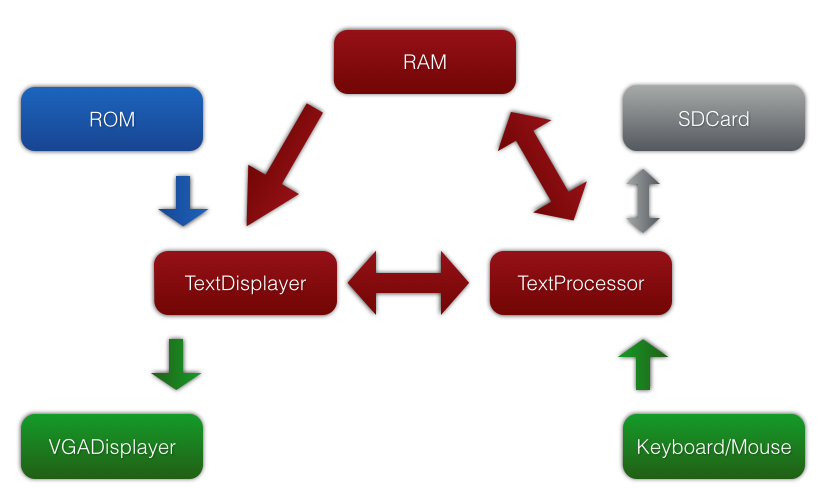
\includegraphics[width=\textwidth]{wordpad1.png}

% section 整体设计 (end)

\section{关键技术分析} % (fold)
\label{sec:关键技术分析}
设计最重要的两个模块分别是TextProcessor和TextDisplayer,以下分别阐述设计要点。

\subsection{TextDisplayer}
\subsubsection{文本显示}
文本的显示成为一开始遇到的最大问题。如果是固定大小的文字的话,很容易计算当前坐标对应的字符位置。但是我们的文本大小是可变的,就造成了一定的困难。最开始的想法是按顺序把每个字的显示内容写入SRAM,但这样一方面很慢,另一方面显示时也需要读取SRAM,读和写的协调难以控制,就放弃了这个想法。后来的想法是扫描RAM中的文本,计算每一个字的坐标,直到碰到当前的坐标,但这样每显示一个像素都要扫描一遍,显然是不现实的。

仔细观察可以发现像素的显示是连续递增的,那么我们就可以根据显示像素的移动动态的维护当前的字符位置,这个位置也是连续递增的。实现中考虑的因素主要是新的一行开始要回滚到当前行最初的字符,或者使用下一行文字,当前扫描坐标超出字符右边界以后要更新当前字符位置,遇到换行符要停止显示字符的移动。

每次显示新的字符时,就根据ROM中预先设定的结构和文本的ASCII码、格式来计算它的ROM偏移,读取显示。为了便于实现,字符的每一行都按照16位对齐,不足16位用0补齐。

\subsubsection{按钮显示}
按钮显示本身十分简单,只要给按钮的ROM一个地址就可以了。但是这样做会导致毛刺的出现,甚至会影响文本区域的显示。后来的做法是预读当前显示按钮,即每当一个按钮显示完以后,就把ROM的地址线置为下一个按钮要显示的内容地址,这样在显示的空白间隙ROM有充足的时间读取内容,并稳定输出。

\subsubsection{MIF文件生成}
显示主要用到了不同字体、大小、字符所产生的MIF文件,以及按钮的MIF文件。为了节约ROM空间,每一个像素点仅存储0或1,颜色会根据具体情况控制显示。MIF文件的生成使用了一个Python脚本。

字符的MIF文件采用大小、字体的方式索引,先存放小号的所有文本,再存放大号。

% section 关键技术分析 (end)

\subsection{TextProcessor}
TextProcessor主要的问题是接受鼠标、键盘事件,处理RAM中的文本。设计中的难点主要有以下:

\subsubsection{光标位置的维护}
由于我们要实现鼠标在文本区域的点击来移动光标位置,以及通过拖动鼠标选中文本,我们都需要知道鼠标当前放在哪个字符上面。对于TextProcessor这个任务比较困难,因为它并不控制显示。一个想法是每次需要鼠标位置时扫描文本并计算,但这样无疑十分繁琐、缓慢。思考后发现只要TextDisplayer在扫描到鼠标对应的坐标时,它当前显示的字符就是鼠标下方的字符!所以鼠标的位置信息用TextDisplayer就可以方便地维护。

\subsubsection{文本的插入}
文本的插入在RAM中需要将当前位置之后的内容后移一位,然后再放入要插入的字符,这可以通过状态机来实现。同时其它的删除、设置格式都类似。插入的状态机如下图:

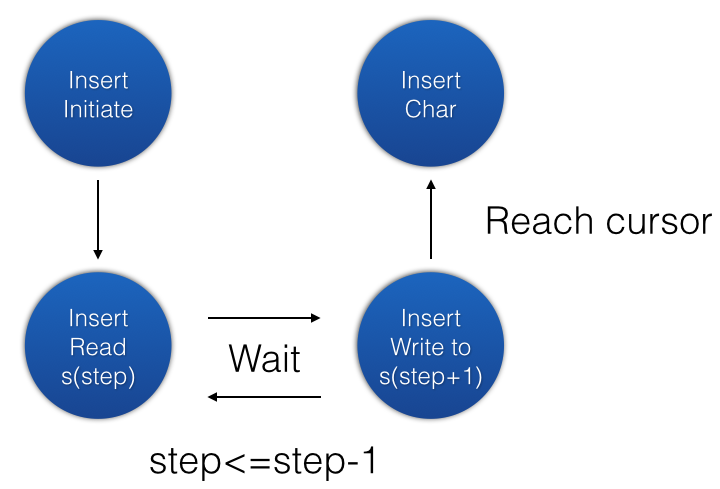
\includegraphics[width=0.8\textwidth]{wordpad2.png}

值得注意的问题是最开始我们的状态机始终无法正常工作,经过长时间调试后才发现RAM无法在一个或两个时钟周期之内完成稳定的读或写。知道这个原因,我们就设定了保持时间,只有保持时间足够,才进行状态转移,这样保证了程序的正确运行。在这里稍微吐槽一下,10个时钟周期怎么都无法正常读写啊!!最后设定的是等待100个周期,不过由于时钟本身够快,肉眼根本无法察觉等待时间。但如果文本规模过于庞大,可能会出现显示不同步的情况。

\section{演示说明} % (fold)
\label{sec:演示说明}
首先打开项目,由于Quartus版本不同,可能会丢失管教绑定信息,这是通过Assignments->Import...来导入Wordpad.csv文件,或者打开文件手动导入。

编译烧录后,需要按rst复位,这时就可以使用键盘输入文字了。通过鼠标左键点击可以控制光标,右键拖动可以选中字符。最上方按钮分别为小大号、两种字体、读取保存(没有实现)、表情符模式(隐藏按钮),下一排颜色为设置字符颜色按钮,右边两个矩形表示当前插入字符的颜色和状态机状态。红色的按钮表示当前插入字符的格式。注意,如果出现鼠标卡住的情况,可以按button1(红色的四个按钮最左边的那个)复位鼠标。

% section 演示说明 (end)

\section{致谢} % (fold)
\label{sec:致谢}
感谢全老师对我们项目的建议和提供的代码,对扩展性的建议让我们有的基于RAM的重新设计!

感谢助教老师周末也来实验室知道我们做实验,以及平时的很多帮助!

感谢我的队友楼华哲对我的大力支持!

% section 致谢 (end)


\end{document}